
\section{Capture Groups Optimization}
\label{sec:capture-groups-optimization-virtual-tree}

In the standard PikeVM algorithm, each thread would contain an array containing for every capture
group whether it went through that capturing group during the matching, and if so what was the
starting index and the ending index (if it was already known) of that substring. For example, 
if we have a thread that already matched YYYY-M for the regex
\texttt{(\textbackslash d \{ 4 \})-(\textbackslash d \{ 2 \})-(\textbackslash d \{ 2 \})} 
and was inside the second capturing group, the information inside the array would be
\begin{center}
    \begin{tabular}{|p{1.3cm}|p{1.3cm}|p{1.3cm}|L{2cm}|}
        \hline 
        Group & Content & Substring & Description \\ \hline
        Year & 0:3 & "YYYY" & \\ \hline
        Month & 5:? & Starts at 'M' & {Didn't exit the group yet.} \\ \hline
        Day & ?:? & & {Didn't enter the group yet.} \\ \hline
    \end{tabular}
\end{center}

One of the peculiarities of the JavaScript semantics is the \textbf{Capture Reset} property.
It states that upon entering inside a quantifier (such as an or, a plus, times, etc...), the
information of all capture groups defined inside that quantifier should be cleared. \\

To achieve this, the bytecode of the PikeVM has two operations that are used to modify the data
of the capture groups are :
\begin{itemize}
    \item \texttt{ClearReg\#i}, clears the register of the $i$-th capturing group.
    \item \texttt{SetReg\#i:entry / SetReg\#i:exit}, set the entry or exit index of the $i$-th capturing group. 
\end{itemize}

One of the other instructions relevant for the capture groups in the PikeVM is the \texttt{Fork} instruction,
that allows to duplicate a thread. In that case, all the data for the capturing groups should be duplicated
so both can be cleared or set independently.

This means that any data structure that we could use to maintain the information of the threads for the
capture groups should represent an abstract array of fixed length $K$ that supports setting, clearing and copying.
Here, $K$ represents all the abstract cells, \texttt{\#i:entry} and \texttt{\#i:exit}
correspond to two distinct indices $i, j \in \left[ 0; K - 1 \right]$.

The standard way in the PikeVM to maintain the data of these threads is using an array of length $K$, with the
$O(K)$ time complexity to copy the whole area during a Fork operation, and $O(1)$ operations to clear or set
the values of the array. In total, we would get a time complexity of $O(KN)$ with this algorithm,
where $N$ is the number of operations. In that case, the number of operation is bounded by the size of the
regular expression $|r|$ and the size of the string $|s|$, $N = O(|s||r|)$. The number of capturing groups can
be of the order of $O(|r|)$, which means $K = O(|r||s|)$ and the time complexity is $O(|r|^2|s|)$. 
Since there are at most $|r|$ threads at any point in time, the space complexity is $O(|r|K) = O(|r|^2)$.

\subsection*{Linked List Data Structure}

The previous paper from the lab \cite{systemf_linear_2024} described another possible data structure that would
allow for a better time complexity of $O(|s||r|)$ in exchange for a space complexity of $O(|s||r|)$.

In this data structure, the array is represented by an immutable linked list of all the modifications, where
the head of the linked list represents the latest modification done to the array.

A Fork operation is done by copying the pointer to the head in $O(1)$. The clear and set
operations are applied by creating a new linked list with the head being that operation and the tail the old
linked list.

For examples, let us look at the following operations (starting with an array $A_1$ initially empty).
\begin{center}
    \begin{tabular}{l l}
        \texttt{0:} & $A_2$ \texttt{ := Fork $A_1$} \\
        \texttt{1:} & $A_1$ \texttt{: Set \#1:entry To $2$} \\
        \texttt{2:} & $A_3$ \texttt{ := Fork $A_1$} \\
        \texttt{3:} & $A_1$ \texttt{: Set \#1:exit To $3$} \\
        \texttt{4:} & $A_3$ \texttt{: Set \#2:entry To $4$} \\
        \texttt{5:} & $A_2$ \texttt{: Set \#3:entry To $5$} \\
        \texttt{6:} & $A_1$ \texttt{: Clear \#1} \\
    \end{tabular}
\end{center}

After these $7$ operations, we obtain the following memory representation for the linked lists.
\begin{center}
    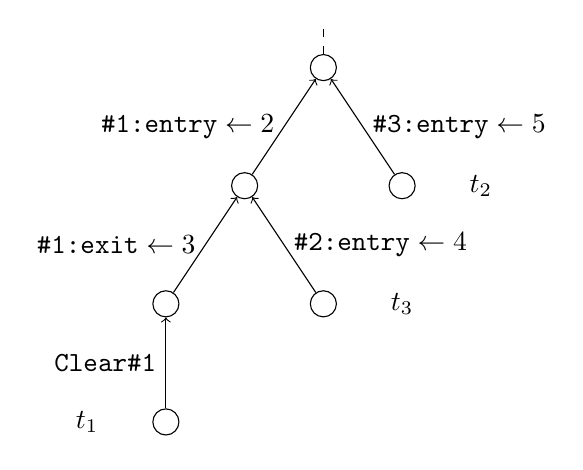
\begin{tikzpicture}
        \node[draw, circle] (root) at (0, 0) {};
        \node[draw, circle] (f_op) at (-1, -1.5) {};
        \node[draw, circle] (s_op) at (-2, -3) {};
        \node[draw, circle] (t_op) at (0, -3) {};
        \node[draw, circle] (m_op) at (-2, -4.5) {};
        \node[left of=m_op] {$t_1$};
        \node[draw, circle] (v_op) at (1, -1.5) {};
        \node[right of=v_op] {$t_2$};
        \node[right of=t_op] {$t_3$};

        \draw[dashed] (root) -- (0, 0.5);
        \draw[->]
            (f_op) -- node[midway, left] (op1) {$\texttt{\#1:entry} \leftarrow 2$} (root);
        \draw[->]
            (s_op) -- node[midway, left] (op2) {$\texttt{\#1:exit} \leftarrow 3$} (f_op);
        \draw[->]
            (t_op) -- node[midway, right] (op3) {$\texttt{\#2:entry} \leftarrow 4$} (f_op);
        \draw[->]
            (m_op) -- node[midway, left] (op4) {$\texttt{Clear\#1}$} (s_op);
        \draw[->]
            (v_op) -- node[midway, right] (op5) {$\texttt{\#3:entry} \leftarrow 5$} (root);
    \end{tikzpicture} \\
    \textit{Linked Lists after all seven operations}
\end{center}

Since there are at most $O(|r||s|)$ such operations and each operation takes both $O(1)$ in time
and space complexity, the total time and space complexity during the matching is $O(|r||s|)$.

\subsection*{Motivation behind optimization}

If we look at the previous example, and imagine now that thread $t_2$ (which owns array $A_2$) fails,
then there would we two parts that we would be interested in optimizing :
\begin{itemize}
    \item The branch from the root to the head of $A_2$, which should be optimized away as this part of the memory
    will never be reused.
    \item The two branches directly above the head of $A_1$ should be optimized into a single link. Indeed,
    it does not make sense to keep that intermediary node as it just takes memory for nothing.
\end{itemize}

Below, these two operations will be respectively called \textbf{Leaf Removal} and \textbf{Branch
Contraction}, and the compressed tree will be called a \textbf{Virtual Tree}.

\subsection*{Virtual Tree}

\begin{definition}
    Let us consider a tree $T = (V, E)$ rooted at the node $r$. The virtual tree
    $\mathcal{V}(T, S)$ for a given subset of nodes of interest $S \subseteq V$
    is defined to be the smallest tree that can be made by applying any number of
    times one of the following operations on $T$ :
    \begin{itemize}
        \item \textbf{Leaf Removal: } Take a leaf $l$ of the rooted tree such that
        $l \not \in S$ and remove that node from the tree.
        \item \textbf{Branch Contraction: } Take a node $n \neq r$ such that it has
        a single child and and such that $n \not \in S$, and remove that node from
        the tree. After that, add an edge between the parent and child of $n$.
    \end{itemize}
\end{definition}

In this definition, the rooted tree represents our initial linked lists,
and the set of nodes $S$ is intended to represent the heads of the active threads.
Our objective will be to maintain only $\mathcal{V}(T, S)$ in
memory instead of keeping the entire tree.

\begin{example}
    \begin{center}
        \begin{tikzpicture}
            \begin{scope}[name prefix=g1, xshift=-2cm]
                \graph [layered layout, components go right top aligned, nodes=draw, edges=rounded corners]
                {
                    r -- a[dashed];
                    a --[blue] b[blue, dashed];
                    b --[blue] d;
                    b --[red] e[red, dashed];
                    a -- c;
                }; 
            \end{scope}
            \begin{scope}[name prefix=g2, xshift=2cm, yshift=-0.5cm]
                \graph [layered layout, components go right top aligned, nodes=draw, edges=rounded corners]
                {
                    r -- {a[dashed] -- {d, c} };
                };
            \end{scope}

            \draw[->] (-1,-1.5) -- (1,-1.5);
        \end{tikzpicture}
         \\
        \textit{Virtual Tree for $S = \left \{ c, d \right \}$}
        \textit{Dashed Boxes represents nodes not in $S \bigcup \left \{ r \right \}$}
        \textit{Red is for Leaf Removal and Blue is for Branch Contraction.}
    \end{center}

\end{example}

\begin{lemma}
    The number of nodes $N$ in the virtual tree $V(T, S)$ is such that :
    $$|S| \leq N \leq 2|S|$$
\end{lemma}

\begin{proof}
    First of all, we can see that every node $x$ that is in $S$ will be in the virtual tree as it can never
    be removed. This implies that the number of nodes will be greater or equal to the size of $S$.

    The proof for the upper bound is omitted here, but can be found on Codeforces \cite{spike1236_virtual_2025}.
    The definition isn't exactly the same but they are equivalent if we assume the root is in the set $S$.
\end{proof}

When a thread $t$ fails with head $h$, we need to remove $h$ from $S$ (this is called a \textbf{Deactivation}).
When we do a Set or Clear operation on a linked list with head $h \in S$, we should create a sub-node $x$ that is
added in $S$ and attached to $h$ (this is called a \textbf{Creation}), and then we need to do a Deactivation on $h$.

\begin{lemma}
    To maintain the virtual tree after one \textbf{Creation} or one \textbf{Deactivation},
    we need to do at most one leaf removal and at most one branch contraction.
\end{lemma}

\begin{proof}
    First of all, when we do a Creation operation, the tree remains a virtual tree and so nothing has to
    be done. When we do a Deactivation, we may need to remove that node if it is a leaf, but then the
    parent can't be both a leaf and not in $S$ (otherwise we would have removed it with a branch contraction).
    Finally, we may need to do a branch contraction on the node or on the parent if it was removed as a leaf.
    After that, no other modification is needed as this does not impact the adjacent node (their degree does
    not change, and their presence/absence in $S$ does not change).
\end{proof}

These two lemmas show us that we can maintain a compressed version of the linked lists
that has $O(|S|)$ nodes. Since our set $S$ is supposed to represent the head of the
linked lists of the active threads and since there are $O(|r|)$ active threads at any point in time, that
compressed version of the linked list has $O(|r|)$ nodes at any point in time. 

\subsection*{Squashing Modifications}

It remains to show what to do with the modifications on the branches that we contract.
If we look at the smallest possible example with a single linked list with two modifications,
there isn't much that can be done except keeping the two modifications in a list (here, a
doubly-linked list).

\begin{center}
    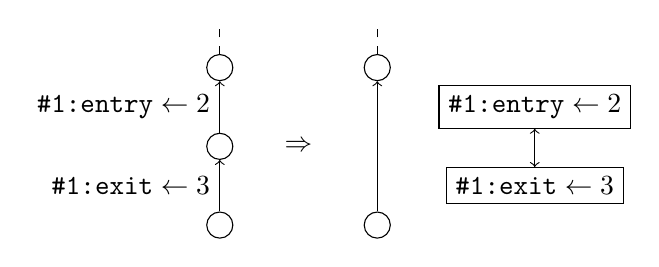
\begin{tikzpicture}
        \node[draw, circle] (root) at (0, 0) {};
        \node[draw, circle] (f_op) at (0, -1) {};
        \node[draw, circle] (s_op) at (0, -2) {};

        \draw[dashed] (root) -- (0, 0.5);
        \draw[->]
            (f_op) -- node[midway, left] (op1) {$\texttt{\#1:entry} \leftarrow 2$} (root);
        \draw[->]
            (s_op) -- node[midway, left] (op2) {$\texttt{\#1:exit} \leftarrow 3$} (f_op);
        
        \node (arrow) at (1, -1) {$\Rightarrow$};

        \node[draw, circle] (root2) at (2, 0) {};
        \node[draw, circle] (s_op2) at (2, -2) {};
        
        \node[draw] (op12) at (4, -0.5) {$\texttt{\#1:entry} \leftarrow 2$};
        \node[draw] (op22) at (4, -1.5) {$\texttt{\#1:exit} \leftarrow 3$};

        \draw[dashed] (root2) -- (2, 0.5);
        \draw[->]
            (s_op2) -- (root2);
        \draw[->] (op12) -- (op22);
        \draw[->] (op22) -- (op12);
        
    \end{tikzpicture}
\end{center}

Such a doubly-linked list will be called an \textbf{Incomplete Form}, as it represents
a sparse version of the modifications.

If an Incomplete Form has a length greater than $K$
the number of cells in our abstract array, then we know that it must have some redundant
information (in particular by the pigeonhole principle, there will be a memory cell that
has at least two operations on it, the latest one being the only one useful).

In that case, we will apply a \textbf{Flattening} operation to create an array of length $K$ that
contains the modifications per cell. Here, if $K = 2$, then the flattened version of the
doubly linked list would be

\begin{center}
    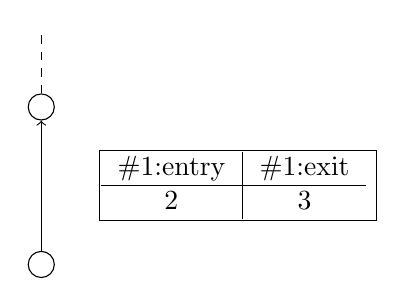
\begin{tikzpicture}
        \node[draw, circle] (root) at (0, 0) {};
        \node[draw, circle] (s_op) at (0, -2) {};
        
        \node[draw, inner sep=0.5pt, align=center] (op1) at (2.5, -1) {
            \begin{tabular}{c|c}
                \#1:entry & \#1:exit \\ \hline
                $2$ & $3$ \\
            \end{tabular}
        };

        \draw[dashed] (root) -- (0, 1);
        \draw[->]
            (s_op) -- (root);
    \end{tikzpicture}
\end{center}

This denser data structure will be called a \textbf{Complete Form}.

Combining two incomplete forms take $O(1)$ time as it is equivalent to concatenating
two doubly linked lists, which is done easily by changing the pointers. If a flattening
is needed (e.g. the length of the new doubly linked list is greater or equal to $K$),
then that flattening will take $O(K)$ time as this can be done by creating an array of
length $K$ and iterating over the doubly linked list (which has size less than $2K$
since it is the concatenation of two linked lists of size less than $K$).

Combining an incomplete form and a complete form can be done in $O(L)$, where $L$ is the
length of the incomplete form by iterating over it. Combining two complete forms
can be done in $O(K)$ by iterating over one of the two complete forms.

\subsection*{Complexity}

\begin{lemma}
    The above solution has a $O(|r|^2)$ space complexity.
\end{lemma}

\begin{proof}
    The size of the virtual tree is $O(|r|)$, and thus it has at most $O(|r|)$ edges.
    A complete form uses $O(K) = O(|r|)$ memory, and an incomplete form of length $L$ uses
    $O(L)$ memory. But we know by construction that $L < K$ and so an incomplete form uses
    $O(K) = O(|r|)$ memory. This means that the virtual tree is stored in memory with $O(|r|^2)$
    space complexity.
\end{proof}

\begin{lemma}
    The above solution has a time complexity of $O(|r||s|)$.
\end{lemma}

Before proving that, we define a tool for the analysis of the complexity, a potential $\Psi$.
In exchange for $O(T)$ in the time complexity of an operation, we can increment $\Psi$ by $T$
(e.g. store $T$ time for the future). Then, we can take $0 \leq T \leq \Psi$ whenever we want
and decrement $\Psi$ by $T$ whilst doing $O(T)$ operations (e.g. retrieve some of the stored
time from the potential). That way, the operation can be amortized over time.

\begin{proof}
    To prove that fact, we will have two potential functions, $\Psi_I$ and $\Psi_C$. $\Psi_I$
    represents the sum of the lengths of the incomplete forms in the virtual tree. $\Psi_C$
    represents $K = O(|r|)$ times the number of complete forms in the virtual tree.
    
    When a creation is done, this creates a new incomplete form with one modification and increments
    $\Psi_I$ by $1$, and so this is in $O(1)$ time complexity.
    
    \begin{itemize}
        \item When a combination happens between two incomplete forms, this is in $O(1)$ and does
        not change the potentials. If a flattening is necessary, it will decrement $\Psi_I$ by
        $L > K$ (we remove an incomplete form of length at least $K$). The flattening is done
        in $O(K)$, and then $\Psi_C$ is incremented by $K$ which costs a total of $O(K)$ time,
        amortized by the $L > K$ from $\Psi_I$. The complexity is therefore $O(1)$.
        \item When a combination happens between an incomplete form of length $L$ and a complete form,
        $\Psi_I$ is decremented by $L$ and $\Psi_C$ stays constant. The combination takes $O(L)$ time,
        but since $L$ was taken from $\Psi_I$, this operation takes $O(1)$ time.
        \item When a combination happens between two complete form, it takes $O(K)$ times and decrements
        $\Psi_C$ by $K$ and so it also takes $O(1)$ time.
    \end{itemize}

    All these operation happen in $O(1)$ amortized and so the total complexity is $O(|r||s|)$ since there
    are at most that many operations on the data structure.
\end{proof}
